\documentclass[a4paper]{../phyreport}
\expName{单双缝实验}
\expDate{2024}{4}{4}
\subDate{2024}{4}{11}
% \expAddr{致原楼206}
% 实验预习处: http://172.31.80.102:7101/
% 快乐制表网站: https://www.tablesgenerator.com/#
\usepackage{makecell}
\usepackage{subfigure}

\begin{document}
\phyExpCover{}
\section{实验设计方案}
\subsection{实验目的}

\begin{enumerate}
  \item 了解衍射的基本概念,探讨狭缝衍射的特征;
  \item 探讨缝宽、缝距、缝数对衍射条纹的影响;
  \item 学习使用PASCO's 850数据接口和Capstone软件进行数据采集和处理。
\end{enumerate}

\subsection{实验原理}
\subsubsection{衍射的基本概念及原理}

波穿过狭缝或圆盘之类的障碍物后会发生不同程度的弯散传播,产生明暗相间的复杂图样。这现象称为衍射。

\paragraph{惠更斯-菲涅尔原理}
波前的每一点发出次波,这些次波互相干涉,叠加形成新的波前。这个原理同时适用于远场极限和近场衍射。

\begin{figure}[H]
  \centering
  \begin{minipage}[t]{0.40\textwidth}
    \centering
    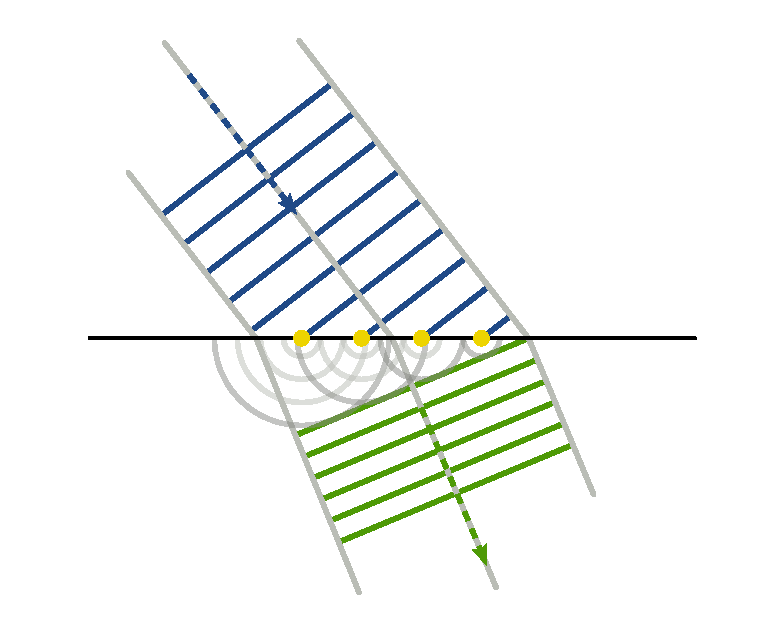
\includegraphics[width=0.7\textwidth]{fig/Refraction_-_Huygens-Fresnel_principle.pdf}
    \caption{波从一个介质传播到另外一个产生折射}
  \end{minipage}
  \qquad
  \begin{minipage}[t]{0.40\textwidth}
    \centering
    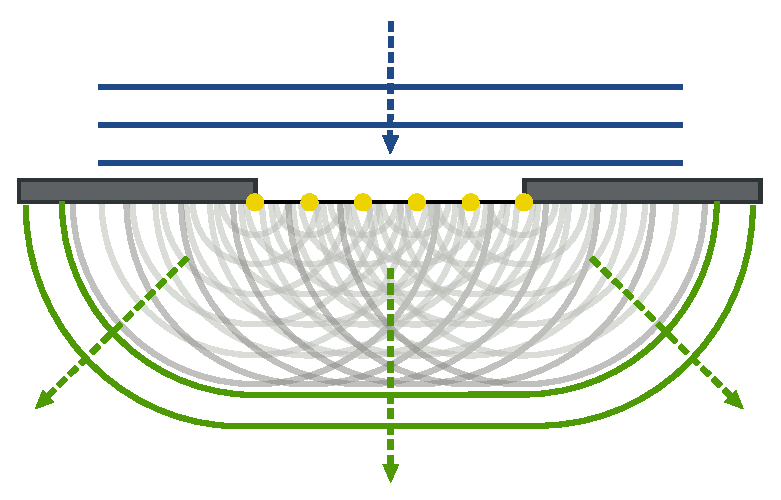
\includegraphics[width=0.7\textwidth]{fig/Refraction_on_an_aperture_-_Huygens-Fresnel_principle.pdf}
    \caption{波遇到障碍物时会产生衍射}
  \end{minipage}
\end{figure}

\paragraph{巴比涅原理}

巴比涅原理指出,两个互补的衍射屏(即一个屏幕是另一个的补充,如一个是孔洞而另一个是相应的障碍物)单独产生的衍射场的复振幅之和等于没有衍射屏时的情况。这个原理在解决复杂衍射问题时非常有用。

\paragraph{衍射条件}

衍射现象的显著性取决于波长 $\lambda$ 与障碍物特征尺寸 $a$ 的比值( $\lambda/a$ )。

\begin{itemize}
  \item $\lambda/a\ge 1$时,衍射效应过于强烈,向散射过渡;
  \item $1/100 < \lambda/a < 1/10$时,衍射现象明显;
  \item $\lambda/a < 1/1000$时,衍射现象很弱,光近乎直线传播,有边缘衍射效应;
  \item $\lambda/a \to 0$时,衍射现象消失,光波按几何光学规律传播。
\end{itemize}

\paragraph{衍射分类}
衍射可按照不同的标准进行分类
\subparagraph{按光路分类} 菲涅耳衍射、夫琅禾费衍射

\subparagraph{按屏分}
单缝衍射、多缝衍射、圆孔衍射、圆屏衍射、直边衍射、光栅衍射……

\subsubsection{单缝衍射}

本实验主要利用图\ref{装置光路} 研究单缝衍射。图中,$\alpha$是缝宽,$\theta$是衍射角,$S$是光源。

\begin{figure}[H]
  \centering
  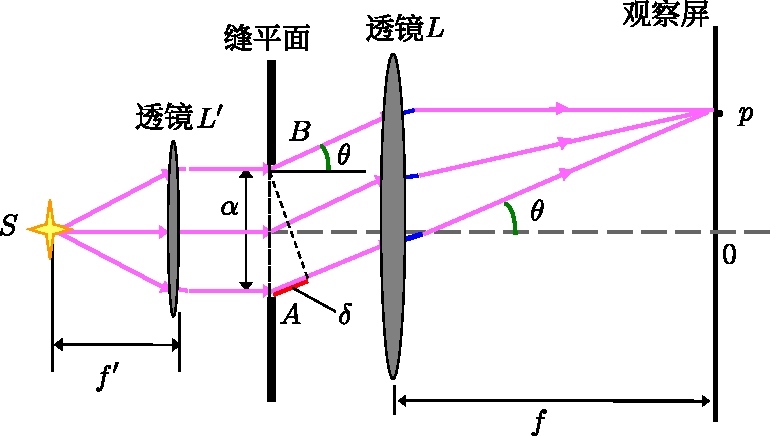
\includegraphics[scale=0.65]{fig/装置光路.pdf}
  \caption{单缝衍射实验装置光路} \label{装置光路}
\end{figure}

对有一条缝的不透明挡板,照射单色平行光,观察其后的光屏。由几何光学,观察屏上只会有一条与狭缝轮廓相同的亮条纹。然而,可以发现在亮条纹两侧,分布着对称的亮条纹。这样现象就是如图\ref{单缝衍射示意图} 演示的衍射。

\begin{figure}[H]
  \centering
  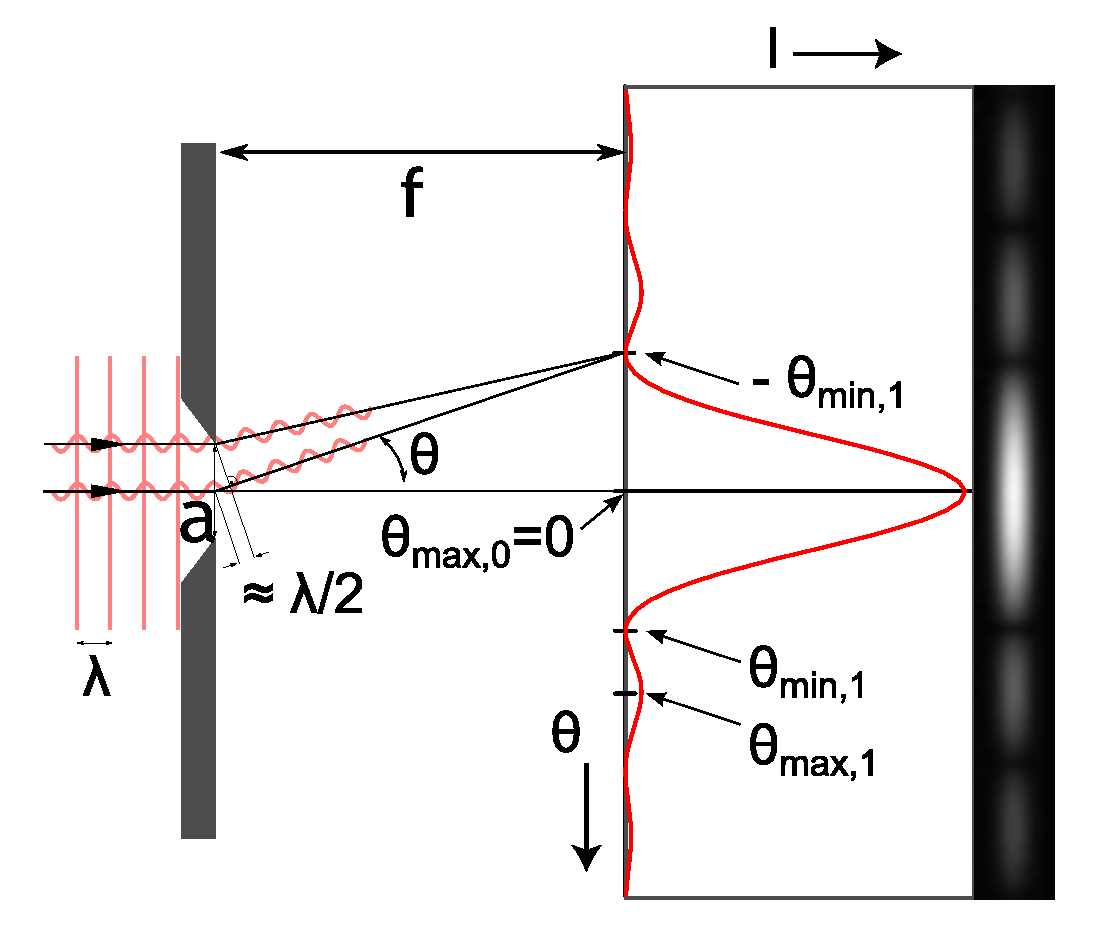
\includegraphics[width=0.45\textwidth]{fig/Single_Slit_Diffraction_First_Minimum.pdf}
  \caption{单峰衍射示意图}
  \label{单缝衍射示意图}
\end{figure}
图右半部分为观察屏水平方向的辐照度分布,辐照度曲线第一个零点$\theta _{min,1}$称为“第一极小值”;图左半部分为单缝衍射示意图,狭缝处点光源发出的光波以角度$\theta$传播到达第一极小值。我们假设这些光束与狭缝垂直平分线的夹角均为$\theta$,基于$L$远大于$d$的前提。

当狭缝宽度大于光波波长,光穿过狭缝向挡板后区域传播并发生干涉。狭缝缝宽之间均匀分布着点光源,衍射图样是点光源共同作用结果。简化分析,入射光具单一波长、单色光,在波源位置相位相同。狭缝后任意位置,光是所有点光源“次光波”在那位置叠加结果。次光波经过路径不同,光程不同,在给定点的相位不同。对任意两个点光源,若次光波在观察屏给定点的相对相位为$2\pi$,则会干涉相长;若相对相位为$\pi$,则会干涉相消。
% 这可找到衍射光强的极大值或极小值,在衍射图样中表现为明暗条纹。

\paragraph{菲涅耳半波带法}

菲涅耳半波带法是单缝衍射中一种简易的分析方法,将平行入射光分成 $k$等分
% ,其中
\begin{itemize}
  \item 入射光半波长的偶数倍:$d\,\sin \alpha =2k(\lambda /2)$,对应暗纹中心。
  \item 入射光半波长的奇数倍:${\displaystyle d\,\sin \alpha =(2k+1)(\lambda /2)}$,对应明纹中心。
\end{itemize}
中央明纹的宽度: 
\begin{equation}
  \label{equ:中央明纹宽度}
  \Delta x = 2 \frac{f \lambda}{a}
\end{equation}
其余明纹的宽度:
\begin{equation}
  \Delta x_i =  \frac{f \lambda}{a}
\end{equation}

\paragraph{理论计算}

一束平行光的波动方程可以表达为

\begin{equation}
  y = A_0 \cos \omega t
\end{equation}

当光穿过缝宽为$a$的单缝上,由Huygens–Fresnel原理,同一波面发出的子波是相干波,
空间$P$点的振幅是这些子波干涉的结果。设想我们把单缝处的波面$AB$分成$N$个
等宽度波带,则单缝可看作$N$各宽度为$a/N$的狭缝的组合,相邻狭缝到$P$
点的光程差为$\Delta = \dfrac{a}{N}\sin \theta $ ,相位差为
$\delta = \dfrac{2 \pi a \sin \theta }{N \lambda}$,则各个狭缝到$P$ 点的振动方程为:第$i$个狭缝:
\begin{equation}
y_i=\dfrac{A_0}{N}\cos[\omega t + (i -1)\delta]
\end{equation}
例如,通过第一个狭缝:$y_1=\dfrac{A_0}{N}\cos \omega t$。

$P$点光场的振动方程为:
\begin{equation}
  y_P=\sum_{i=1}^{N}\frac{A_0}{N}\cos[\omega t + (i -1)\delta]
\end{equation}

\paragraph{单缝衍射强度公式}

\begin{align}
  \text{振幅分布} \qquad  & \tilde{E}(P)  =A\frac{\sin u}{u},  \quad u=\frac{\pi a \sin \theta}{\lambda} \\
  \text{强度分布}  \qquad & I =I_0 \frac{\sin^2 u}{u^2}, \quad \delta = \frac{2 \pi a \sin \theta}{N \lambda}
\end{align}

规定相邻暗纹的角距离为其间明纹的角宽度中央主极大的半角宽度为:$\Delta \theta = \lambda / a$

\subsubsection{多缝衍射}

\paragraph{单缝衍射对多缝衍射的调制作用}

多缝在$P$点产生的复振幅是N个振幅相同、相邻光束程差相等的多光干涉结果,即考虑两方面:每个单缝各自的衍射,及缝与缝之间的干涉。

\begin{align}
  P \text{点振幅} & \qquad \tilde{E}(P) = A\dfrac{\sin u}{u}\dfrac{\sin\dfrac{N}{2}\delta}{\sin\dfrac{\delta}{2}}\exp\left[i(N-1)\dfrac{\delta}{2}\right], \quad u=\frac{\pi a \sin \theta}{\lambda} \\
  P \text{点光强} & \qquad I_0 = \left(\dfrac{\sin u}{u}\right)^2\left(\dfrac{\sin\dfrac{N}{2}\delta}{\sin\dfrac{\delta}{2}}\right)^2, \quad \delta = \frac{2 \pi}{\lambda} d \sin \theta
\end{align}

其中$u$是单缝衍射因子,$\delta$是多光束干涉因子。多光束干涉使得光强成等间距明暗条纹,单缝衍射使得光强外部包络成单缝衍射的形状,单缝单缝衍射对多缝衍射具有调制作用。

多缝衍射中存在缺级现象,这主要是由多缝干涉的强度极强点与单缝衍射的强度极弱点重合造成。具体来说,$\theta$满足下面条件时,就会出现缺级现象。

对多缝干涉,明纹满足的光栅方程:
\begin{equation}
  d \sin \theta = m \lambda, \qquad m=0, \pm 1, \pm 2\dots
\end{equation}
式中,$m$为主极大的级次,$\theta$为衍射角,$d$为缝距。

对于单缝衍射,暗纹满足条件:
\begin{equation}
  a \sin \theta = n \lambda, \qquad  m=0, \pm 1, \pm 2\dots
\end{equation}
式中,$\theta$为衍射角,$a$为缝宽。

如果干涉的主极大和衍射的极小值重合时会产生缺级,缺级的干涉级为$m=n\dfrac{d}{a}$

对于多缝夫琅和费衍射,缝间距$d$影响各级主极大的位置,缝宽a影响光强在各级主极大间的分配,共同影响着衍射图样。

\subsection{实验仪器}

\subsubsection{实验装置}

\begin{figure}[H]
  \centering
  \begin{tikzpicture}[font=\small]
    \draw[] (0, 0) rectangle (10,0.5);
    \node[left] at (0, 0.25) {底座};

    \draw[] (1, 0.5) -- (1,0.75);
    \draw[] (0.7, 1) rectangle (1.3, 0.75);
    \node[left] at (0.75, 0.875) {纵向滑轨与移动传感器};
    \draw[] (0.5, 0.6) -- (1.5, 1.15);

    \draw[] (0.8, 1) rectangle (1.2, 1.5);
    \node[left] at (0.75, 1.25) {光传感器};
    \draw[fill=white] (1.2, 1.25) circle [radius=0.1];
    \draw[] (8.5, 0.5) -- (8.5,1);
    \draw[] (8.25, 1) rectangle (8.75, 1.5);
    \draw[] (8.4, 1.25) -- (8.6, 1.25);

    \node[left] at (8.25, 1.25) {衍射狭缝(单缝/多缝)};

    \draw[] (9.5, 0.5) -- (9.5,1);
    \draw[] (9.25, 1) rectangle (9.75, 1.5);
    \draw[<-] (9.25, 1.25) -- (9.75, 1.25);
    \node[right] at (9.75, 1.25) {激光器};
  \end{tikzpicture}
  \caption{实验装置示意图}
\end{figure}

\subsubsection{选用仪器列表}

\begin{table}[H]
  \centering
  \caption{选用仪器列表}
  \begin{tabular}{ll}
  \toprule
  仪器名称                & 用途          \\
  \midrule
  850接口 UI-5000             & 用于采集和处理数据     \\
  计算机和PASCO Capstone  & 用作数据采集平台和数据处理工具 \\
  衍射狭缝(单缝) & 用于产生衍射效应 \\
  衍射狭缝(多缝) & 用于产生衍射效应 \\
  激光发生器 & 用作衍射光的光源\\
  光传感器 & 用于检测衍射光的强度 \\
  转动传感器和线性转换器 & 用于移动光传感器的位置并记录数据 \\
  光阑 & 用于调节入射光的强度 \\
  \bottomrule
  \end{tabular}
\end{table}

\longLine
\section{实验内容及具体步骤}
实验步骤如下
\subsection{测量步骤}\label{测量步骤}
\begin{enumerate}
\item 将激光器放置在底座边缘,狭缝放置在靠近激光器位置
\item 将组装好的线性转换器和光传感器固定在底座另一边缘
\item 调整激光器-狭缝-传感器水平
\item 打开850接口,打开计算机Capstone软件,连接传感器,以位置为横坐标,相对光强为纵坐标准备绘图
\item 在以下不同实验中,调整狭缝后:
\begin{enumerate}
    \item 开始记录数据
    \item 将光传感器从线性转换器的一端以合适速度移动到另一端
\end{enumerate}
\end{enumerate}

\subsection{单缝衍射工作任务}

\subsubsection{探究缝宽$a$对衍射的影响}

\begin{enumerate}
    \item 使用\ref{测量步骤} 中的方法观测0.02mm,0.04mm,0.08mm,0.16mm的衍射条纹
    \item 记录衍射条纹图像与中央明纹、一级明纹、二级明纹的宽度、强度
    \item 定量讨论缝宽对条纹的影响。
\end{enumerate}

\subsection{多缝衍射工作任务}

\subsubsection{研究单缝衍射对多缝干涉条纹的调制作用,观察缺级。}

\begin{enumerate}
    \item 使用缝宽相同的单缝与多缝(0.04mm缝宽),观测衍射条纹
    \item 要求单缝衍射+多缝干射条纹图像;标注缺级的位置 
\end{enumerate}

\subsubsection{研究缝距对多缝干射的影响}

\begin{enumerate}
    \item 自行选择参数,自行选择记录数据。
    \item 记录多缝干射条纹图像;记录条纹的宽度、强度,做定量分析
\end{enumerate}

\subsubsection{研究缝数对多缝干射的影响}

\begin{enumerate}
    \item 观察0.04mm的2、3、4、5缝图像
    \item 记录多缝干射条纹图像;记录条纹的宽度、强度,做定量分析
\end{enumerate}

% \longLine
% \longLine
\section{数据记录及数据处理}

\subsection{单缝衍射实验:探讨缝宽$a$对衍射的影响}
\paragraph{实验数据图像}
测得不同宽度的单缝衍射从仪器获得图像如下:

\begin{figure}[H]
  \centering
  \begin{minipage}[b]{0.45\linewidth}
    \centering
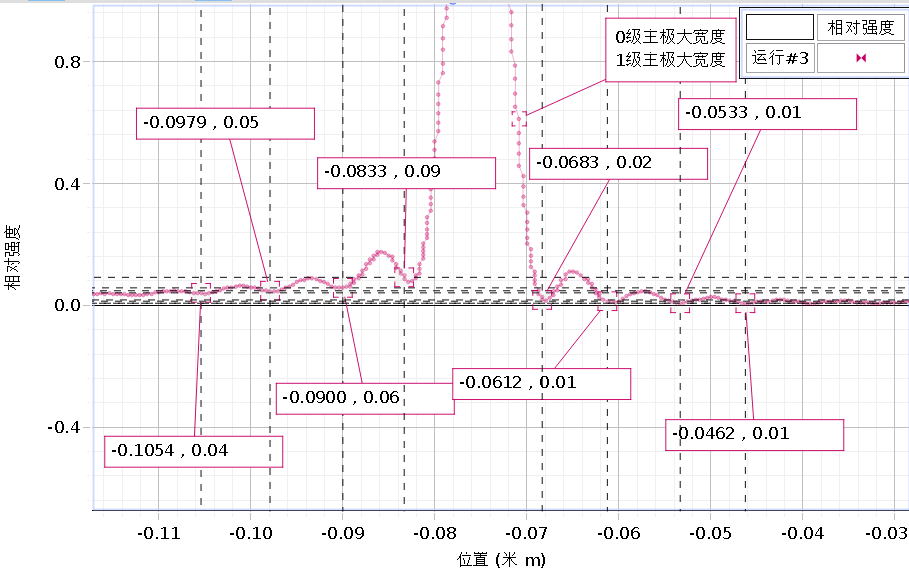
\includegraphics[width=0.9\linewidth]{fig/单峰/0.02.png}
\captionof{subfigure}{0.02mm缝宽}
  \end{minipage}
  \begin{minipage}[b]{0.45\linewidth}
    \centering
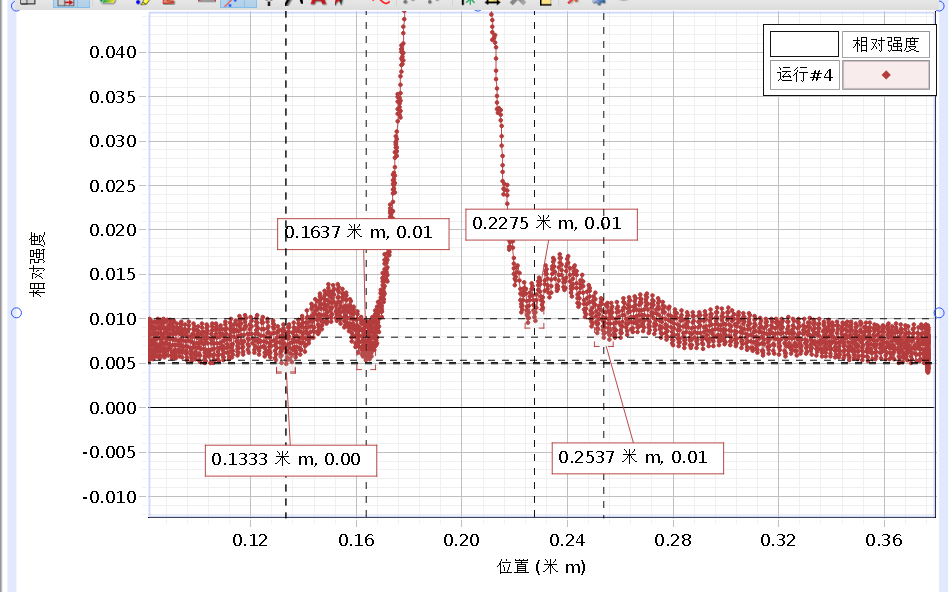
\includegraphics[width=0.9\linewidth]{fig/单峰/0.04.png}
\captionof{subfigure}{0.04mm缝宽}
  \end{minipage}
  \begin{minipage}[b]{0.45\linewidth}
    \centering
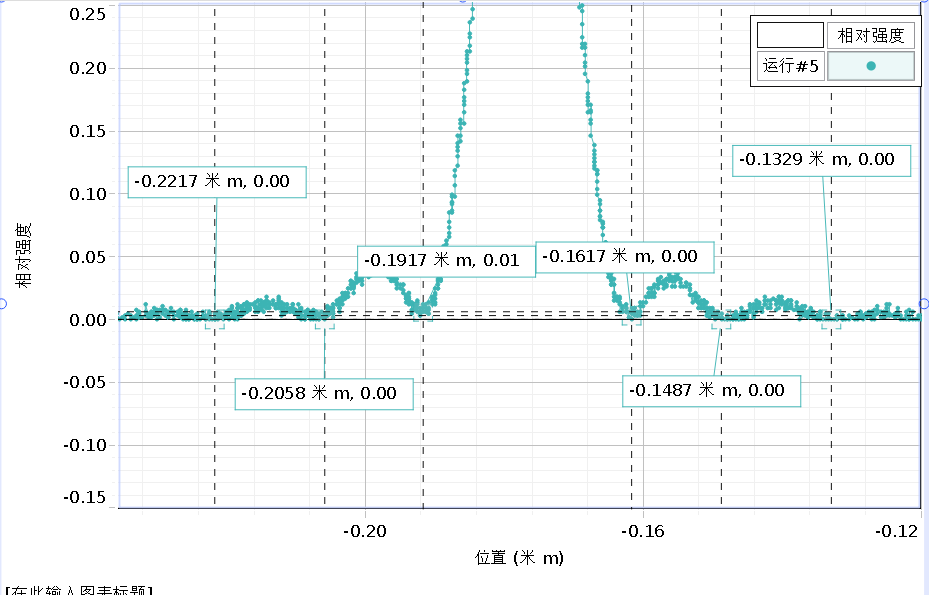
\includegraphics[width=0.9\linewidth]{fig/单峰/0.08.png}
\captionof{subfigure}{0.08mm缝宽}
  \end{minipage}
  \begin{minipage}[b]{0.45\linewidth}
    \centering
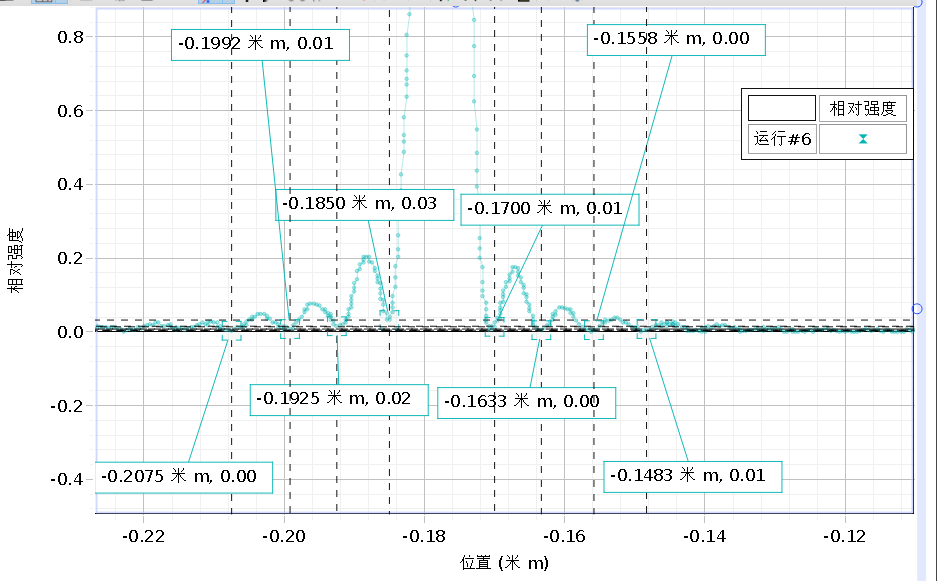
\includegraphics[width=0.9\linewidth]{fig/单峰/0.16.png}
\captionof{subfigure}{0.16mm缝宽}
  \end{minipage}
  \caption{不同缝宽下的相对光强随位置变化的图像}
  \label{单缝}
\end{figure}

% 使用 MATLAB 仿真得到下图:
% \begin{figure}[H]
%   \centering
%   \begin{minipage}[b]{0.45\linewidth}
%     \centering
% 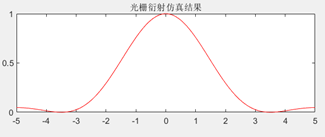
\includegraphics[width=0.9\linewidth]{fig/仿真/0.02.png}\label{fig:subfig1}
% \captionof{subfigure}{0.02mm缝宽}
%   \end{minipage}
%   \begin{minipage}[b]{0.45\linewidth}
%     \centering
% 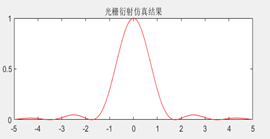
\includegraphics[width=0.9\linewidth]{fig/仿真/0.04.png}\label{fig:subfig2}
% \captionof{subfigure}{0.04mm缝宽}
%   \end{minipage}
%   \begin{minipage}[b]{0.45\linewidth}
%     \centering
% 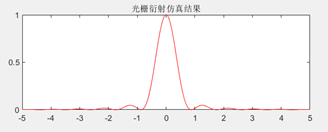
\includegraphics[width=0.9\linewidth]{fig/仿真/0.08.png}\label{fig:subfig3}
% \captionof{subfigure}{0.08mm缝宽}
%   \end{minipage}
%   \begin{minipage}[b]{0.45\linewidth}
%     \centering
% 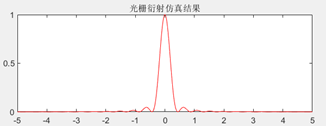
\includegraphics[width=0.9\linewidth]{fig/仿真/0.16.png}\label{fig:subfig4}
% \captionof{subfigure}{0.16mm缝宽}
%   \end{minipage}
%   \caption{不同缝宽下的相对光强随位置变化的仿真图像}
%   \label{单缝仿真}
% \end{figure}
% % 可以观察到,
% 仿真结果与实验结果基本吻合。

\paragraph{数据处理}
总结测得不同宽度单缝数据如下表:

\begin{table}[H]
  \centering
  \caption{不同宽度单缝数据(单位:mm)}
    \begin{tabular}{rrrrr}
    \toprule
    \multicolumn{1}{l}{缝宽$a$} & \multicolumn{1}{l}{最大相对光强} & \multicolumn{1}{l}{中心明纹$\Delta x$} & \multicolumn{1}{l}{1级明纹$\Delta x_1$} & \multicolumn{1}{l}{2级明纹$\Delta x_2$} \\
    \midrule
    0.02  & 0.97  & 150.00  & 71.00  & 79.00  \\
    0.04  & 1.12  & 63.80  & 30.40  & 29.70  \\
    0.08  & 3.50  & 30.00  & 14.10  & 15.80  \\
    0.16  & 10.60  & 15.00  & 10.00  & 7.50  \\
    \bottomrule
    \end{tabular}%
  \label{tab:不同宽度单缝数据}%
\end{table}%

进一步计算$\frac{\Delta x}{\Delta x_1},\quad \Delta x \cdot a$,整理得到:

% \begin{table}[H]
%     \centering
%     \caption{不同单缝宽度相关数据计算结果}
%     \begin{tabular}{rrr}
%         \toprule
%         缝宽(mm) &  $\frac{\Delta x}{\Delta x_1}$ & $ \Delta x \cdot a$\\
%         \midrule 
%         0.16 & 2.01 & 2.53\\
%         0.08 & 2.04 & 2.49\\
%         0.04 & 1.85 & 2.30\\
%         0.02 & 2.32 & 2.16\\
%         \midrule
%         平均值 & 2.05 & 2.37\\
%         标准差 & 0.19 & 0.17\\
%         变异系数 & 9.3\% & 7.2\%\\
%         \bottomrule
%     \end{tabular}
% \end{table}
% Table generated by Excel2LaTeX from sheet 'Sheet2'
\begin{table}[H]
  \centering
  \caption{不同单缝宽度相关数据计算结果}
    \begin{tabular}{rrr}
    \toprule
    缝宽(mm) & $\frac{\Delta x}{\Delta x_1}$ & $ \Delta x \cdot a$\\
    \midrule
    \multicolumn{1}{r}{0.02} & 2.11  & 3.00  \\
    \multicolumn{1}{r}{0.04} & 2.10  & 2.55  \\
    \multicolumn{1}{r}{0.08} & 2.13  & 2.40  \\
    \multicolumn{1}{r}{0.16} & 1.50  & 2.40  \\
    \midrule
    平均值   & 1.96  & 2.59  \\
    标准差   & 0.27  & 0.25  \\
    \bottomrule
    \end{tabular}%
  \label{tab:不同单缝宽度相关数据计算结果}%
\end{table}%

\paragraph{数据分析}
由表\ref{tab:不同宽度单缝数据} ,随着缝宽越大,最大相对光强越高;中心明纹宽度明显减小
,体现衍射引起的光斑扩散效果随着缝宽减小而增强
;一级和二级明纹宽度随缝宽减小而增加
,体现了缝宽对衍射光斑扩散的影响。
% $\frac{\Delta x_0}{\Delta x_1} \approx 2$,与理论结果基本吻合;
% $ \Delta x \cdot a$ 约为一定值,与理论结果$ \Delta x\cdot a = 2 f \lambda$ 基本吻合。
由表\ref{tab:不同单缝宽度相关数据计算结果}发现,
$\frac{\Delta x}{\Delta x_1}$与$ \Delta x \cdot a$ 为定值,与理论结果2相符。
\subsection{多缝衍射实验:研究缝距对多缝干涉的影响}

选取缝宽$a=0.04mm, 0.08mm$与缝距$d=0.25mm, 0.50mm$双缝组合,得到:

\begin{figure}[H]
  \centering
  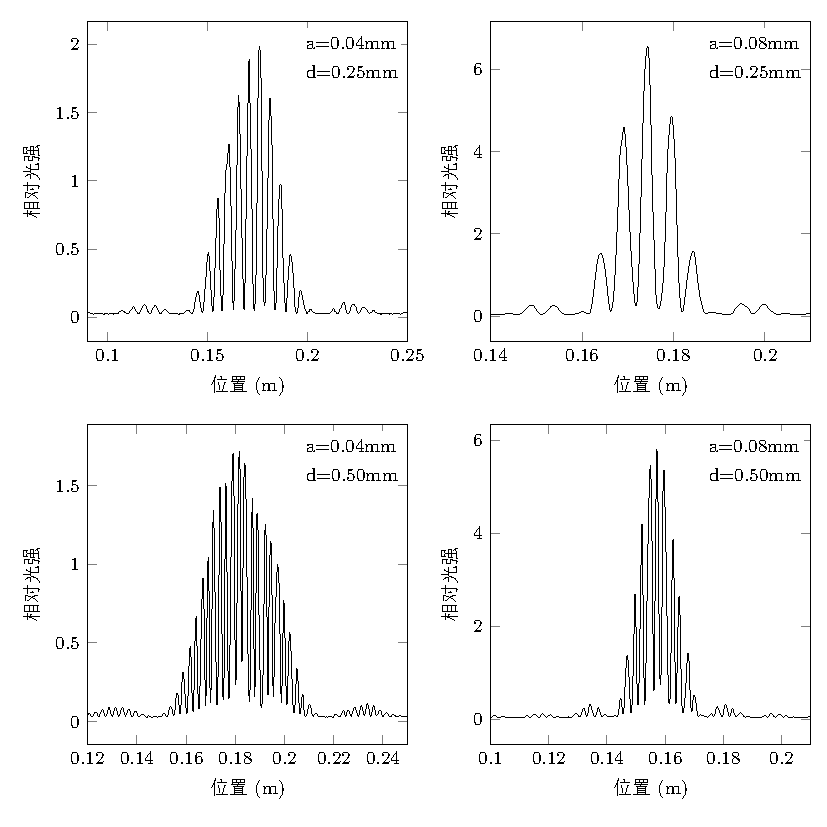
\includegraphics[]{fig/多缝/双峰改变ad4图.pdf}
  \caption{不同缝距缝宽产生的不同干涉条纹} \label{缝间距}
\end{figure}
% Table generated by Excel2LaTeX from sheet 'Sheet2'

\paragraph{数据处理}
测量所得图像中亮纹的极大值与间距,得到以下表格:

\begin{table}[H]
  \centering
  \caption{不同缝宽缝距下的衍射条纹数据,单位(mm)}
    \begin{tabular}{clr}
    \toprule
    \multicolumn{1}{l}{缝宽$a$} & 缝距$d$   & 明纹宽度$\Delta x$\\
    \midrule
    \multirow{2}[2]{*}{0.08} & 0.50 & 2.0 \\
          & 0.25 & 5.4 \\
\cmidrule{1-2}    \multirow{2}[2]{*}{0.04} & 0.50 & 2.5 \\
          & 0.25 & 5.1 \\
    \bottomrule
    \end{tabular}%
  % \label{tab:addlabel}%
\end{table}%H
进一步计算$d \Delta x$得下表:

\begin{table}[H]
  \centering
  \caption{不同缝距数据计算表,单位(mm)}
    \begin{tabular}{rlr}
    \toprule
    缝宽$a$ & 缝距$d$   & $d \Delta x$ \\
    \midrule
    \multicolumn{1}{c}{\multirow{2}[2]{*}{0.08}} & 0.50 & 1.00 \\
          & 0.25 & 1.35 \\
\cmidrule{1-2}    \multicolumn{1}{c}{\multirow{2}[2]{*}{0.04}} & 0.50 & 1.25 \\
          & 0.25 & 1.28 \\
    \midrule
          & 平均值   & 1.22  \\
          & 标准差   & 0.13  \\
    \bottomrule
    \end{tabular}%
  \label{tab:不同缝距数据计算表}%
\end{table}%
\paragraph{数据分析}
从表\ref{tab:不同缝数下的明纹宽度与光强数据} 可以看出,随着缝距增大,最大相对光强不变,亮纹间距减小;
从表\ref{tab:不同缝距数据计算表}看出,$d \Delta x $ 为在误差允许范围内可视为定值,与理论结果相符。
\paragraph{MATLAB 仿真}用以上参数,得到下图:
\begin{figure}[H]
  \centering
  \begin{minipage}[b]{0.45\linewidth}
    \centering
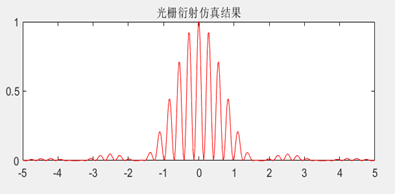
\includegraphics[width=0.9\linewidth]{fig/仿真/0.040.25.png}
\captionof{subfigure}{$a=0.04mm,d=0.25mm$}
  \end{minipage}
  \begin{minipage}[b]{0.45\linewidth}
    \centering
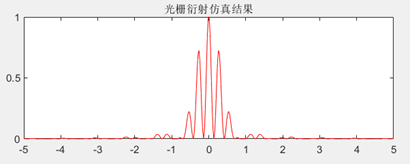
\includegraphics[width=0.9\linewidth]{fig/仿真/0.080.25.png}
\captionof{subfigure}{$a=0.08mm,d=0.25mm$}
  \end{minipage}
  \begin{minipage}[b]{0.45\linewidth}
    \centering
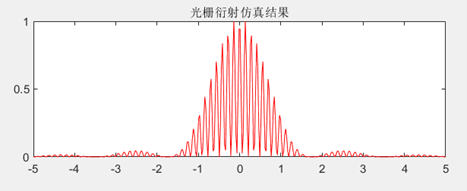
\includegraphics[width=0.9\linewidth]{fig/仿真/0.040.50.png}
\captionof{subfigure}{$a=0.04mm,d=0.50mm$}
  \end{minipage}
  \begin{minipage}[b]{0.45\linewidth}
    \centering
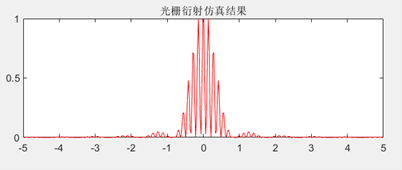
\includegraphics[width=0.9\linewidth]{fig/仿真/0.080.50.png}
\captionof{subfigure}{$a=0.08mm,d=0.50mm$}
  \end{minipage}
  \caption{不同缝距下的仿真图像}
  % \label{单缝}
\end{figure}
实验与仿真一致.
% 分析表格数据:
% 从表\ref{tab:不同缝数下的明纹宽度与光强数据} 可以看出,随着缝距增大,最大相对光强不变,亮纹间距减小;
% 从表\ref{tab:不同缝距数据计算表}看出,$d \Delta x $ 为在误差允许范围内可视为定值,与理论结果相符。

\subsection{单缝衍射对多缝干涉条纹的调制作用}
理论中,单缝衍射对多缝干涉条纹的调制作用,会产生缺级。

此处,
将双缝衍射图像与单缝衍射图像(a = 0.04mm,  d = 0.50mm)重叠,其中实线为双缝干涉的图像,虚线为单缝衍射的图像,得到下图:
\begin{figure}[H]
  \centering
  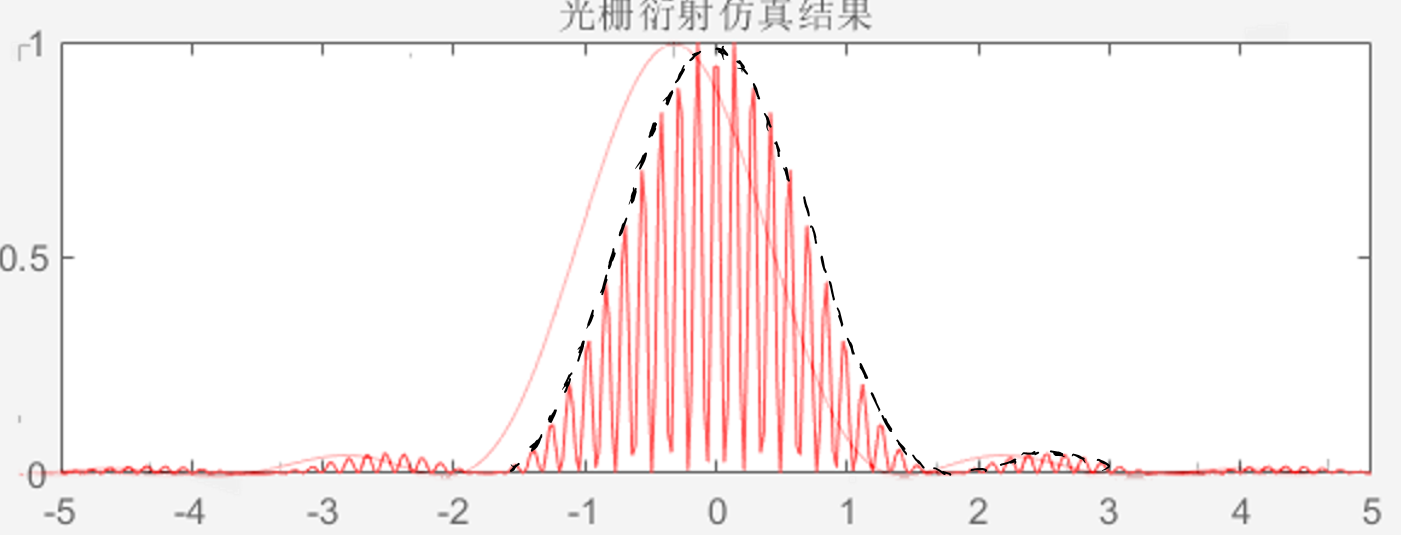
\includegraphics[width=0.6\linewidth]{fig/仿真/组合.png}
  \caption{双缝衍射与单缝衍射图像的叠加}
\end{figure}

% 可以观察到右侧单缝与双缝重合处的缺级。
图中,可看出单缝干涉的图像包络多缝干涉的图像,单缝对多缝的干涉条纹的调制作用缺级的位置为单缝干涉的极小值理论相吻合。
% 展示了单缝对多缝的干涉条纹的调制作用,可得单缝干涉的图像包络多缝干涉的图像,缺级的位置为单缝干涉的极小值理论相吻合.

\subsection{研究缝数与多缝干涉关系}
\paragraph{多缝干涉图像}
固定缝宽$a=0.04mm$,缝间距$d= 0.125mm$,取缝数为2,3,4,5,得到:
\begin{figure}[H]
  \centering
  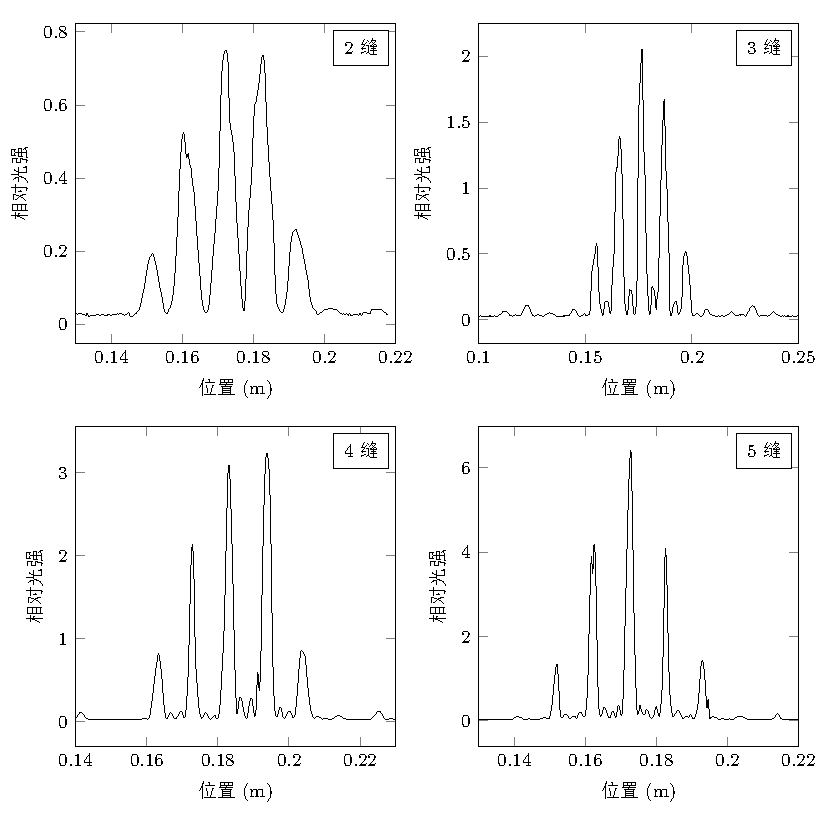
\includegraphics[]{fig/多缝/多缝2345tikz.pdf}
    \caption{不同缝数下的干涉条纹图像} \label{缝数}
\end{figure}

图中次高峰,2缝没有,3缝1个,4缝2个,5缝3个。总结出次极大的数量为$N-2$。

\paragraph{光强与缝数} 进一步计算 $I / N^2$,得到下表:
\begin{table}[H]
  \centering
  \caption{不同缝数下的明纹宽度与光强数据}
    \begin{tabular}{ccc}
    \toprule
    缝数$N$  & 最大相对光强$I$ & $I / N^2$ \\
    \midrule
    2  & 0.75  & 0.19  \\
    3  & 2.20  & 0.24  \\
    4  & 3.20  & 0.20  \\
    5  & 6.70  & 0.27  \\
    \midrule
          & 平均值   & 0.22  \\
          & 标准差   & 0.03  \\
    \bottomrule
    \end{tabular}%
  \label{tab:不同缝数下的明纹宽度与光强数据}
\end{table}%

从表\ref{tab:不同缝数下的明纹宽度与光强数据} 可以看出,随着缝数的减少,明纹宽度增加,最大相对光强减小。具体来说,从5缝到2缝时,明纹宽度从4.06增加到10.42,最大相对光强从4.68减少到0.79。
这表明,随着缝数减少,光的强度分布趋于分散,每个条纹的亮度也随之减弱。此外,实验中 $\frac{I}{N^2}$ 的值在误差范围内保持不变,与理论一致。

\paragraph{MATLAB 仿真}使用参数,得到下图
\begin{figure}[H]
  \centering
  \begin{minipage}[b]{0.45\linewidth}
    \centering
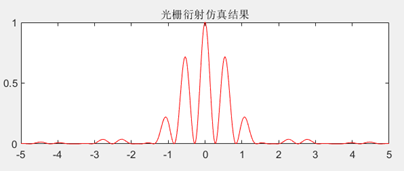
\includegraphics[width=0.9\linewidth]{fig/仿真/2.png}
\captionof{subfigure}{2峰仿真}
  \end{minipage}
  \begin{minipage}[b]{0.45\linewidth}
    \centering
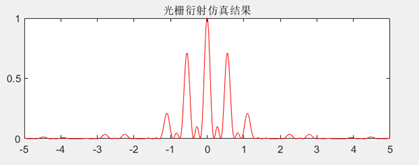
\includegraphics[width=0.9\linewidth]{fig/仿真/3.png}
\captionof{subfigure}{3峰仿真}
  \end{minipage}
  \begin{minipage}[b]{0.45\linewidth}
    \centering
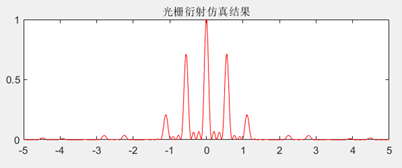
\includegraphics[width=0.9\linewidth]{fig/仿真/4.png}
\captionof{subfigure}{4峰仿真}
  \end{minipage}
  \begin{minipage}[b]{0.45\linewidth}
    \centering
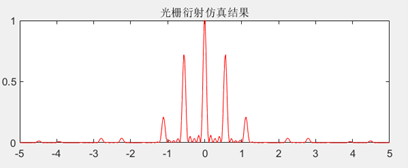
\includegraphics[width=0.9\linewidth]{fig/仿真/5.png}
\captionof{subfigure}{5峰仿真}
  \end{minipage}
  \caption{不同缝数仿真图像}
  \label{fig:不同缝数仿真}
\end{figure}
仿真结果与实验结果基本吻合。

\subsection{误差分析}
本实验主要观察,但获取数据的过程中可能存在的误差有:
\begin{itemize}
    \item 光污染干扰,测得光强不为实际光强,影响准确性
    \item 仪器精度限制可能导致测量值与理论值存在偏差。
    \item 在测量明纹宽度时,判断明纹边缘的主观性可能引入误差。
\end{itemize}

\paragraph{减小误差方法}
\begin{itemize}
  \item 暗室遮光
  \item 使用合适精度仪器,并引入校准过程
  \item 利用计算机自动寻找谷值,测量明纹宽度
\end{itemize}

% \longLine
\section{实验结果陈述与总结}
\subsection{结果陈述}
% \paragraph{单缝衍射实验结果}

%     本次实验得出了在不同缝宽下的干涉条纹图像(图\ref{单缝} )。
%     实验数据显示,随着缝宽的减小,最大相对光强显著降低,表明较窄的缝宽导致通过缝隙的光强度减弱。
%     缝宽的减小还导致中心明纹宽度显著增加,说明衍射引起的光斑扩散效果随着缝宽减小而增强。一级和二级明纹宽度的增加进一步证实了缝宽对衍射光斑扩散的影响。
%     计算得到的$\frac{\Delta x}{\Delta x_1}$与$\Delta x \cdot a$值显示,中心明纹宽度与一级明纹宽度的比约为2,且$\Delta x \cdot a$约为一定值,与理论预测基本吻合。

% \paragraph{多缝衍射实验结果}

%     本次实验观察到了多缝与单缝条纹的叠加,观察到了缺级(图\ref{缺级} );获得了在缝数改变与缝间距改变时的不同干涉条纹图像(图\ref{缝数} 和 图 \ref{缝间距} )。
%     在多缝干涉中,随着缝数的减少,明纹宽度增加,相对最大光强减小。这一结果表明,缝数较少时,干涉效应减弱,导致单个明纹占据更宽的空间,而光强度分布变得更加分散。
%     实验还研究了缝距对多缝干涉的影响。结果表明,当缝距增大时,亮纹间距减小,但最大相对光强基本不变。$d \Delta x$的计算结果在误差范围内可视为定值,符合理论预期。
%     观察到的干涉图像中,次极大的数量为$N-2$,其中$N$为狭缝数量。

%     4.1.1缝宽a对衍射光强,中央明纹宽度的影响,发现光强与a成正相关比,中央明纹宽度光宽与a成反比。
%     4.1.2单缝衍射对多缝干涉条纹的调制作用,观察到缺级为对应单缝衍射的极小值。
%     4.1.3缝距对多缝干射的轮廓不影响,但是与条纹宽度成反比
%     4.1.4缝数对多缝干射的影响,观察到次主峰的个数与缝数N关系为N-2,中央光强大小与缝数N的关系为N2,中央条纹宽度与N成反比。
综合而言,本次实验深入了解了衍射现象,并得出了单缝和多缝衍射中光强和条纹特征的规律。    
\paragraph{单缝衍射实验}随着缝宽的减小,我们观察到最大相对光强显著降低,同时中心明纹宽度增加,这表明较窄的缝宽导致光强度减弱和衍射光斑扩散效果增强。我们的计算结果显示,中心明纹宽度与一级明纹宽度的比约为2,与理论预测基本吻合。
\paragraph{多缝衍射实验}观察到了多缝与单缝条纹的叠加,以及缺级现象。随着缝数的减少,明纹宽度增加,相对最大光强减小,这表明干涉效应减弱,单个明纹占据更宽的空间,光强度分布更加分散。缝距的增大导致亮纹间距减小,但最大相对光强基本不变,这符合理论预期。同时,我们观察到次极大的数量与缝数的关系为$N-2$,中央光强大小与缝数的关系为 $N^2$ ,中央条纹宽度与缝数成反比。

\subsection{实验总结}

本次实验通过探讨衍射的基本概念及狭缝衍射的特征,以及调查缝宽、缝距和缝数对衍射条纹的影响,深入了解了这一物理现象。使用PASCO 850数据接口和Capstone软件进行数据采集和处理,为实验增添了很大的价值,并为今后的物理学习和对物理现象的认知提供了重要支持。

实验中利用仪器测光强分布,得出了单缝和多缝衍射的规律,展现了计算机配合仪器的便捷性和准确性。值得注意的是,实验还揭示了单缝干涉对多缝干涉的调制作用。总的来说,本次实验进行顺利,从最初对仪器的陌生到熟练使用,期间也经历了细致的实验过程,力求避免重复实验,为实验结果的准确性提供了保障。


\endBox
\end{document}
